% -*- root: ../thesis.tex -*-

\chapter[Application-Level Scheduling]{Programming and Deployment of Active Objects with Application-Level Scheduling%
\footnote{This work is partially supported by the EU FP7-231620 project: HATS.}}
% 
\label{ch:p01:ch01}
% 
\chapterauthor{Behrooz Nobakht, Frank S. de Boer, Mohammad Mahdi Jaghoori,  Rudolph Schlatte}

\section*{Abstract}
% Active objects provide a natural means for programming distributed systems.
We extend and implement a modeling language based on concurrent active objects with application-level
scheduling policies.
The language allows a programmer to assign priorities at the application level, for example,
to method definitions and method invocations, and assign corresponding  policies to the individual active objects
for scheduling the messages.
Thus, we   leverage scheduling and performance related issues,
which are becoming increasingly important in multi-core and cloud  applications, from the underlying operating system to the application level.
We describe a tool-set to transform models of active objects extended with application-level
scheduling policies  into Java.
This tool-set allows a direct  use of Java class libraries; thus,  we
obtain  a full-fledged programming language
based on active objects which allows for high-level control of deployment related issues.

\subparagraph*{Conference Publication}
\emph{Proceedings of the 27th Annual ACM Symposium on Applied Computing -- ACM SAC 2012, Pages 1883--1888, DOI \smalltt{10.1145/2245276.2232086}}

% \category{D.1.3}{Programming Techniques}{Concurrent Programming}
% \category{D.2.3}{Software Engineering}{Coding Tools and Techniques}
% \category{D.3.0}{Programming Languages}{General}
% \terms{Languages, Design}
% \keywords{Application-level scheduling, ~Priority scheduling, ~Creol, Java, Actor model, Concurrent active objects}

\section{Introduction} \label{sec:introduction}
One of the major challenges in the design of programming
languages is to provide high-level support for  multi-core and cloud  applications which are becoming increasingly important.
Both multi-core and cloud  applications require an explicit and precise treatment of non-functional properties, e.g., resource requirements.
On the cloud, services execute in the
context of virtual resources, and the amount of resources actually available to a service is subject to change.
Multi-core applications require techniques 
to help the programmer optimally use potentially many cores. At
the operating system level, resource management is greatly affected by scheduling which
is largely beyond the control of most existing high-level programming languages.
Therefore, for optimal use of the available resources, we cannot avoid leveraging
scheduling and performance related issues from the underlying operating system
to the application level. However, the very nature of high-level languages is to
provide suitable abstractions that hide
implementation details from the programmer. The main challenge in designing programming languages
for  multi-core and cloud  applications
is to find a balance between these two conflicting requirements.

We investigate in this paper how concurrent active objects in a high-level object-oriented
language can be used for high-level scheduling of resources. We use the notion of
concurrent objects in Creol \cite{creol:broch_owe,mpd:andrews}. A
concurrent object in Creol has control over one processor; i.e. it has a
single thread of execution that is controlled by the object itself.
Creol processes never leave the enclosing object; method invocations
result in a new process inside the target object.  Thus, a concurrent
object provides a natural basis for a deployment scheme where each
object virtually possesses one processor. Creol further provides high-level
mechanisms for synchronization of the method invocations in an object;
however, the scheduling of the method invocations are left
unspecified. Therefore, for the deployment of concurrent objects in
Creol, we must, in the very first place, resolve the
basic scheduling issue; i.e. which \textit{method} in which
\textit{object} to select for execution.
We show how to introduce priority-based scheduling of the messages of the individual objects
at the application-level itself.


In this paper we also propose a 
% pluggable and extensible 
tool
architecture to deploy Creol applications. To prototype the tool
architecture, we choose Java as it provides low-level concurrency features, i.e., threads, futures, etc.,
required for multi-core deployment of object-oriented applications. The tool
architecture prototype transforms Creol's constructs for concurrency to their
equivalent Java constructs available in the
{\jtt{java.util.\-concurrent}} package. As such, Creol provides
a high-level structured programming discipline based on active objects on top of Java.
Every active object in Creol is transformed to an object in Java that uses a priority manager
and scheduler to respond to the incoming messages from other objects. Besides,
through this transformation, we allow the programmer to seamlessly use, in the
original Creol program, Java's standard library including all the data types.
Thus, our approach converts Creol from  a modeling language to a full-fledged
 ``programming'' language.

Section \ref{sec:creol} first provides an overview of the Creol language with application-level scheduling. 
In Section \ref{sec:compiler}, we elaborate on the design  of the tool-set and the
prototype. The use of the tool-set is exemplified by a case study in Section \ref{sec:caseStudy}.
Section \ref{sec:relwork} summarizes the related work. 
Finally, we conclude in Section \ref{sec:conclusion}.

%\section{Preliminaries: Creol} \label{sec:creol}
%

% The (simplified) syntax of Creol is given in Fig.~\ref{fig::creolSyntax}.
% Here we introduce the basic concepts of Creol.
%
%
% \newcommand{\trans}[1]{\,{\stackrel{{#1}}{\longrightarrow}}\,}
% \newcommand{\gtrans}[2]{\,{\stackrel{{#2}}{\longrightarrow_{#1}}}\,}
% \newcommand{\transtwo}[1]{\, { \stackrel {{  \stackrel{{#1}}{\longrightarrow} }} {{#1}} }   \,}
% \newcommand{\M}{\mathcal{M}}
% \newcommand{\Nat}{\mathbb N}
% \newcommand{\Act}{\Sigma}
% \newcommand{\id}[1]{\mathit{#1}}
% 
% \begin{figure}[t]
% \begin{center}
% \begin{tabular}{l@{~~~}l}
% \begin{math}
% \begin{array}{lcl}
% \id{IF} & ::= & \id{\bf interface}\ N
% %\{[\{N\}_,^+]\}^?
% \{(\id{Par})\}^?
% %\\~&~&
% \{\id{\bf inherits}\ \id{Inh}\}^?  \\
% ~   & ~ &  \id{\bf begin}\ \{\id{\bf with}\ \id{N}\ \id{Msig}^+\}^?\ \id{\bf end} \\
% %\id{Type} & ::= & N\{[\{\id{Type}\}_,^+]\}^? \\
% \id{Inh}  & ::= & \{\id{N}\{(E)\}^?\}_,^+ \\
% \id{Par} & ::= & \{\{v\}_,^+ :\id{N}\}_,^+ \\
% \id{Msig} & ::= & \id{\bf op}\ N \{(\{\id{\bf in}\ \id{Par}\}^?\ \{\id{\bf out}\ \id{Par}\}^?)\}^? \\
% \id{CL} & ::= & \id{\bf class}\ N
% %\{[\{N\}_,^+]\}^?\
% \{(\id{Par})\}^?
% \\
% ~&~&
%  \{\id{\bf contracts}\ \id{Inh}\}^? \  \{\id{\bf inherits}\ \id{Inh}\}^?  \\
% ~ & ~ & \id{\bf begin} \ \id{Vdcl}^? \{\{\id{\bf with}\ \id{N}\}^?\ \id{Mtd}\}^*\ \id{\bf end} \\
% \id{Vdcl} & ::= & \id{\bf var}\ \{\{v\}_,^+: \id{N}\{=e\}^?\}_,^+ \\
% \end{array}
% \end{math}
% &
% \begin{math}
% \begin{array}{l}
% \id{Mtd} ::= \{\id{Msig} ==\{\id{Vdcl};\}^? \ S\}^+ \\
% g\ ::=\ b\ |\ t?\ |\ \lnot g\ |\ g \land g \\
% p\ ::= \ x.m \ |\ m \\
% S\ ::=\ \epsilon\ | \ s;S \\
% s\ ::=\ (S)\ |\ V := E\ |\ \id{\bf skip} \\
% ~~~~~ |\ v := \id{\bf new}\ N(E)\ | \ !p(E) \\
% ~~~~~ | \ t!p(E) \ | \ t?(V)\ | \ p(E;V) \\
% ~~~~~ | \ \id{\bf if}\ b\ \id{\bf then}\ S\ \id{\bf else}\ S\ \id{\bf end}\\
% ~~~~~ | \ \id{\bf await}\ g \ | \ \id{\bf await}\  t?(V)\\
% ~~~~~ | \ \id{\bf await}\  p(E;V)\ |\ \id{\bf release} \\
% \end{array}
% \end{math}
% \end{tabular}
% \end{center}
% \caption{BNF grammar for Creol. Curly
% brackets are used as meta parenthesis, superscript ? for optional
% parts, superscript * for repetition zero or more times, whereas
% $\{. . .\}_,^+$  denotes repetition one or more times with �,� as delimiter. Identifiers N denote interface, class, type, or method names.
% %The language syntax for method definitions, with typical
% %terms for each category.
% Capitalized terms such as $E$, $V$, and $S$,
% denote lists of the syntactic categories of the corresponding lower-case terms~\cite{johnsen07sosym,JohnsenOY06}.}\label{fig::creolSyntax}
% \end{figure}


Creol~\cite{creol:broch_owe} (Concurrent Reflective Object-oriented Language) is
an object oriented modeling language designed for specifying distributed
systems. A Creol object implicitly has a dedicated processor and thus
encapsulates an execution thread. Different objects communicate only by
asynchronous method calls, i.e., similar to message passing in Actor models
\cite{actors:agha};  however in Creol, the caller can poll or wait for return
values or termination of the called method. This can also be used to simulate
synchronous method calls. % we can say: like RPC We use an exclusive resource
%object as a running example, shown in Listing \ref{lst:exres}.

When an object is created, its local state is initialized by executing the \footnotesizett{init} method.
Then the object starts its active behavior by executing its
\footnotesizett{run} method if defined. % (e.g., in class \footnotesizett{User}). 
When receiving a method call a new process is created to execute the method. 
Methods can have processor release points which define interleaving points explicitly.
When a process is executing, it is not interrupted until it finishes or reaches a release point.
Release points can be conditional:
%, e.g.,  \footnotesizett{await mutex.request()} in Listing \ref{lst:exres} checks for termination of \footnotesizett{request}. 
if the guard at a release point evaluates to true, the
process keeps the control, otherwise, it releases the processor and becomes
disabled as long as the guard is not true. Whenever the processor is free, an
enabled process is {\em nondeterministically} selected for execution, i.e.,
scheduling is left unspecified in Creol in favor of more abstract modeling.


%%%%%%%%%%%%%%%%%%%%%%%%%%%%%%%%%%%%%%%%%%%%%%%%%%%%%%%%%%%%%%%%%%%%%%%%%%%%%%%%%%%%%%%%%%%%%

% \subsection{Creol}
% Creol \cite{creol:web} stands for Concurrent Reflective Object-oriented
% Language. Creol is a language that provides programming constructs and
% reasoning control in the context of open distributed systems
%  taking an object-oriented approach
% \cite{creol:web,creol:broch_owe,mpd:andrews}.
% 
% Johnson and Owe \cite{creol:broch_owe} focus on synchronization of distributed systems
% and the challenges. They argue that it is difficult to combine active and
% passive behavior in concurrent objects; so, they propose Creol as an
% object-oriented language for the solution mainly taking advantage of
% \textit{processor release points} and a notion of \textit{asynchronous method
% call}. Creol is designed to unite object orientation and distribution and helps
% to dynamically change between active and reactive behavior.
% 
% %According to \cite{creol:broch_owe,mpd:andrews}, the basic interaction models
% %for concurrent processors are \textsl{shared variables}, \textsl{remote method
% %calls}, and \textsl{message passing}. Shared variables do not generalize well
% %with distributed environments. In remote method call (RMI), the caller is
% %blocked until the response is received. In contrast, as message passing does not
% %transfer control between concurrent objects is not blocking. Message passing can
% %either be \textit{synchronous} or \textit{asynchronous}. In synchronous mode,
% %both sender and receiver should be ready to take part in the interaction,
% %however, in asynchronous mode, a message can be sent at any time regardless of
% %when the receiver accepts the message.
% 
% Creol's message passing is analogous to Actor Model \cite{actors:agha}. However,
% they \cite{creol:broch_owe} believe that actors do not distinguish replies from
% invocations, so capturing method calls with actors quickly becomes unmanageable.
% In Creol, method calls are taken as the communication primitive for concurrent
% objects. In Creol, an object encapsulates an execution thread.
% %Thus, some data types are not considered objects inside an
% %object such as basic data types. Each object has a unique identity (name)
% %through which the communication with other objects occurs.  Object names are
% %exchanged with one another. 
% 
% Creol is a language by \textsl{interface}. Every object implements an interface
% in the language \cite{creol:broch_owe,creol_overview:blanchette}. Creol
% introduces the notion of \textsl{cointerface} to be used when the callee may
% need to access to caller object. In this case, a \texttt{with} clause is used to
% specify and restrict access to different objects supporting different
% interfaces. 
% 
% %Creol provides inheritance a bit different of what is generally perceived. A
% %\textsl{class} can \texttt{implement} an interface, \texttt{contract} an
% %interface, or \texttt{inherit} a class. The difference lies in the semantics
% %that is passed down to the hierarchy. In case of contracting, the signature of
% %super interfaces are also present in the semantics of the object of the class.
% %However, in the case of inheriting, the semantics of the super class is not
% %passed down \cite{creol_overview:blanchette}.
% 
% In Creol, an asynchronous message can be sent at any time
% \cite{creol:broch_owe}. Also, \textit{method overtaking} is allowed; i.e. if
% some methods offered by some object are invoked in the same order, it is up to
% the object to reorder the \textit{method instances} in execution. When the
% caller needs the return values from the callee, it may ask for it in which case
% it may be suspended based on the processor release points in Creol. Moreover, a
% message can be synchronous causing the caller to suspend till the reply is
% ready. In Creol, a callee does \textit{not} distinguishes synchronous and
% asynchronous invocation.
% 
% Creol introduces the notion of processor release point
% \cite{creol:broch_owe,creol_overview:blanchette} to provide an explicit
% mechanism to release or acquire processing unit during execution. Essentially,
% clause \texttt{await g} releases processor if guard expression \texttt{g}
% evaluates to false and grabs it again later when \texttt{g} is true. Also,
% \texttt{wait} explicitly releases processor. Creol's asynchronous message
% passing takes advantage of such processor release point model.
% 



\lstset{language=Creol,escapeinside={(*}{*)}}



\section{Application-Level Scheduling}
\label{sec:creol}

Creol \cite{creol:broch_owe} is a full-fledged object-oriented language with formal semantics for modeling and analysis of systems of concurrent objects. 
Some Creol features include interface and class inheritance and being strongly typed such that safety of dynamic class upgrades can be statically ensured \cite{yu06fmoods}.
In this section, we explain the concurrency model of Creol using a toy example: an exclusive resource, i.e., a
resource that can be exclusively allocated to one object at a time, behaving as a mutual exclusion token. 
Further, we extend Creol with priority-based application-level scheduling.

The state of an object in Creol is initialized using the \lstinline{init} method.
Each object then starts its active behavior by executing its
\lstinline{run} method if defined. % (e.g., in class \lstinline{User}). 
When receiving a method call, a new process is created to execute the method. 
Creol promotes {\em cooperative} non-preemptive scheduling for each active object. 
It means that a method runs to completion unless it explicitly releases the processor. 
As a result, there is no race condition between different processes accessing object variables. 
%Methods can have processor release points which define interleaving points explicitly.
Release points can be conditional, e.g.,   \lstinline{await }$\sim$\lstinline{taken}. 
If the guard at a release point evaluates to true, the
process keeps the control, otherwise, it releases the processor and becomes
disabled as long as the guard is not true. Whenever the processor is free, an
enabled process is {\em nondeterministically} selected for execution, i.e.,
scheduling is left unspecified in standard Creol in favor of more abstract modeling.

%\Mahdi{Do we want to talk about with clauses?}

To explain extending Creol with priority specification and scheduling, we take a {\em client/server} perspective.
Each {caller} object is viewed as a client for the {callee} object who behaves as a server. 
We define priorities at the level of language constructs like method invocation or definition rather than low-level concepts like processes.

\begin{lstlisting}[float=t, label=lst:exres, caption=Exclusive Resource in Creol %, multicols=2
]
interface Resource begin
	(* \label{lst:priority_range} *)(*
	%with User  \label{lst:with} 
	*)
		op request()
		op release()
end

class ExclusiveResource implements Resource begin
	var taken := false;
	(* \label{lst:priority_class} *)
	op request () == 
		await (*$\sim$*)taken; 			(* \label{lst:await_taken} *)
		taken := true;
	op release () ==
		taken := false
end
\end{lstlisting}


On the server side, an interface may introduce a \textit{priority
range} that is available to all clients. For instance, in Line
\ref{lst:priority_range} of {\footnotesize\texttt{Resource}} in Listing
\ref{lst:exres}, we can define a priority range: 

\begin{lstlisting}[frame=none, numbers=none]
priority range 0..9
\end{lstlisting}


On the client side, method calls may be given priorities within the range specified in the server interface. For example, calling the \ftt{request} method of the \ftt{mutex} object: 

\begin{lstlisting}[frame=none, numbers=none]
mutex ! request() priority(7);
\end{lstlisting}


Scheduling \textit{only} on the basis of client-side priority requirements is too restrictive.
For example, if there are many \ftt{request} messages with high priorities and a low priority \ftt{release}, the server might block as it would fail to schedule the \ftt{release}.
In this particular example, we can solve this problem by allowing the servers to
prioritize their methods.
This involves a declaration of a priority range generally depending on the structure of the class. 
In our example, assuming a range 0..2 added in Line \ref{lst:priority_class}, this requires changing the method signatures in the {\ftt{Exclusive\-Resource}} class: 

\begin{lstlisting}[frame=none, numbers=none]
op request() priority(2) == ...
op release() priority(0) == ...
\end{lstlisting}


This gives \ftt{release}  a higher priority over \ftt{request}, because by default, the smaller values indicate higher priorities.
Furthermore, the server may also introduce priorities on certain 
characteristics of a method invocation such as the kind of ``release statement''
being executed. 
For example, a process waiting at Line \ref{lst:await_taken} could be given a higher priority over new requests by assigning a smaller value:

\begin{lstlisting}[frame=none, numbers=none]
await (*$\sim$*)taken priority(1);
\end{lstlisting}


The priority can be specified in general as an expression; we used here
only constant values.
Evaluation of this expression at runtime should be within the given
range.
If no priority is specified for a method invocation or definition, a
default priority value will be assigned.

% 
% This is an example of {\em method level} priority specification, which is specified inside a class together with the definition of a method. 
% Method definitions without an explicit priority are given a default priority value. 
% %As discussed in Section \ref{sec:conclusion}, 
% Other possible levels of priority include method invocation level, specified by the caller, or interface level priorities. 
% %

We discussed different levels of application-level priorities. 
Note that now each method invocation in
the queue of the object involves a tuple of priorities.
We define a general function $\delta$ as an ``abstract priority manager'':
%
\[ \delta : P_1 \times P_2 \times P_3 \times \ldots \times P_n \longrightarrow  P \]

The function $\delta$ maps the different levels of priority in the object
($\{P_1,\ldots,P_n\}$) to a single priority value in $P$ that is internally used by the
object to order all the messages that are queued for execution. Each
method in the object may have a $\delta$ assigned to it. In an extended
version of $\delta$, it can also involve the internal state of the object,
e.g., the fields of the object. 
In this case, we have dynamic priorities.

For example, in {\ftt{ExclusiveResource}}, we have two different levels of priorities, namely  the client-side and server-side priorities, which range over $P_1 = \{0, \ldots, 9\}$ and $P_2 = \{0, 1, 2\}$, respectively. 
So, we define $\delta: P_1 \times P_2 \rightarrow P$ as:
%
\[
\delta(p_1, p_2) = p_1 + p_2 \times |P_1|
\]

To see how it works, consider a \ftt{release} and a \ftt{request} message, both sent with the client side priority of 5. 
Considering the above method priorities, we have $\delta(5, request) = \delta(5,2) = 25$ and  $\delta(5, release) = \delta(5,0) = 5$.
It is obvious that the range of the final priority value is $P = \{0,\ldots,29\}$.

Note that the abstract priority manager in general does \textit{not} completely
fix the ``choice'' of which method invocation to execute. 
In our tool-set, we include an extensible library of predefined scheduling policies such as strong or weak fairness that further refine the application-specific multi-level priority scheduling. 
The policies provided by the library are available to the user to annotate the classes.
We may declare a scheduling policy for the \ftt{ExclusiveResource} class by adding at Line
\ref{lst:priority_class} in Listing \ref{lst:exres}: 
%
\begin{quote}
\lstinline{scheduling policy StronglyFairScheduler;} 
\end{quote} 

% These scheduling policies will also be represented in terms of a corresponding
% priority range in the $\delta$ function.
% In summary, there will be, first, priorities that directly stem from the
% model and are statically specified by the client or the server and, second, 
% there will be priorities that dynamically change through time based on
% the runtime information of the application. In the latter case, 
A scheduling policy may
use runtime information to re-compute the dynamic priorities and ensure
properties such as fairness of the selected messages; for instance, it may
take advantage of the ``aging'' technique to avoid starvation. 
%Thus, $\delta$ will take into consideration all the different concerns when assigning a final priority value to a message.

%\Mahdi{Starvation?}


\section{Tool Architecture} \label{sec:compiler}


\begin{figure}[t]
\begin{center}
  %\vspace{-.1cm}
  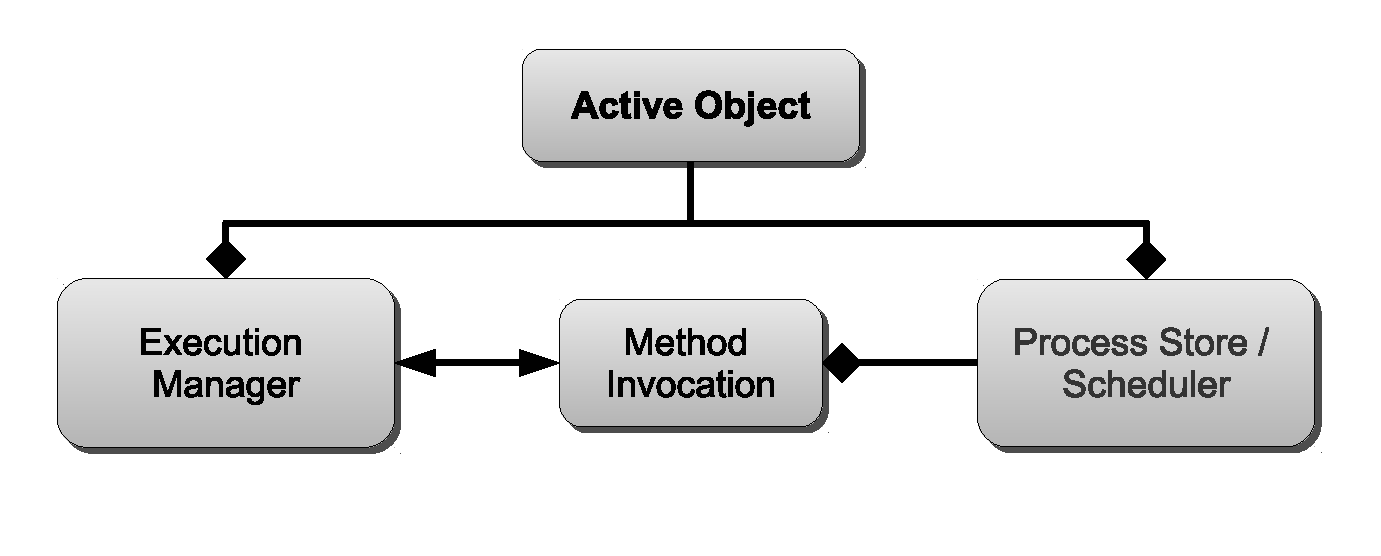
\includegraphics[scale=0.36]{figs/manticore-concurrency-v4}
  \caption{\Crisp Architecture: Structural Overview}
  \label{fig:api}
\end{center}
\end{figure}

We have implemented a tool to translate Creol programs into Java programs for execution, called {\em \Crisp} (Creolized Interacting Scheduling Policies).
\Crisp provides a one-to-one mapping from Creol classes and methods to their equivalent Java constructs. 
In order to implement active objects in Creol, we use the \jtt{java.util.concurrent} package (see Figure \ref{fig:api}).
Each active object consists of an instance of a process store  and an execution manager to store and execute the method invocations. 

Incoming messages to the active object are modeled as instances of \MethodInvocation, a subclass of \jtt{java.util.\-concurrent.FutureTask} that  wraps around the original method call.
Therefore the caller can later get the result of the call.
Additionally, \MethodInvocation encapsulates information such as priorities assigned to the message. 
% Asynchronous messages are stored in the process store as instances of \MethodInvocation. The result of the asynchronous method call can be fetched through the method invocation that encapsulates a future value.
% To support Creol's processor release statements, method invocations provide the
% means to be stopped and resumed. 

The \ftt{ProcessStore} itself uses an implementation of the \ftt{BlockingQueue} interface in \jtt{java.util.concurrent} package. Implementations of \ftt{BlockingQueue} are thread-safe, i.e.,  all methods in this interface operate atomically using internal locks encapsulating the implementation details from the user. 

The \ftt{ExecutionManager} component is responsible for selecting and executing a pending method invocation.
It makes sure that only one method runs at a time, and takes care of processor release points.
%It is implemented using \jtt{java.util.concurrent} in order to provide deployment on multi-core  architectures. We now discuss how in overall an active object operates on a multi-core architecture.

In the following, we explain how the active object behaves in different scenarios, from a ``client/server'' perspective.  
% for the sake of explanation; each active object
% essentially can be seen as a server, in which case all the other objects act as its clients that
% request a method to be executed.

% \subsection{The Problem}
% In this section we briefly sketch the main software engineering problem of deploying 
application-level scheduling of Creol objects onto multicore.


A simple implementation  maps each Creol object unto a single Java thread (e.g., {\jtt{java.lang.Thread}}) which
executes messages taken from a message queue according to some
scheduling policy.  The major drawback of this implementation strategy
is scalability.  OS-level threads are costly resources, and a typical
system written in object-oriented style might instantiate tens of
thousands of objects at runtime.  Thus, any real-world program would
quickly overwhelm current operating systems, see for example our case study in Section \ref{sec:caseStudy}.
Another major software engineering problem of this scheme is that it requires an implementation of  asynchronous method calls 
(e.g., polling/waiting for return values and storing/retrieving local variables).

The basic mechanism of asynchronous method calls is in fact provided by the {\jtt{java.util.\-concurrent}} package by
means of thread pools
which leverage hardware level constructs  to allow a reduction of the overhead of the multi-threaded Java programs by using lock-free, and wait-free thread-safety mechanisms.
This package, e.g., the implementation of {\jtt{FutureTask}}, requires another implementation strategy for a Java backend for Creol which uses
one Java thread per Creol process and allows for a one-to-one translation of Creol classes and methods to Java classes and methods.
However,  one of the major problems in leveraging scheduling issues is that this package does not allow high-level control of the scheduling of the threads.
The main contribution of the paper is the introduction of a general architecture on top of the {\jtt{java.util.\-concurrent}} package
to provide such high-level control for concurrent objects.




% Local Variables:
% mode: LaTeX
% TeX-master: "paper.tex"
% End:



\subsection{A New Method Invocation}
\label{sec:add}

\begin{figure}[t]
%\begin{center}
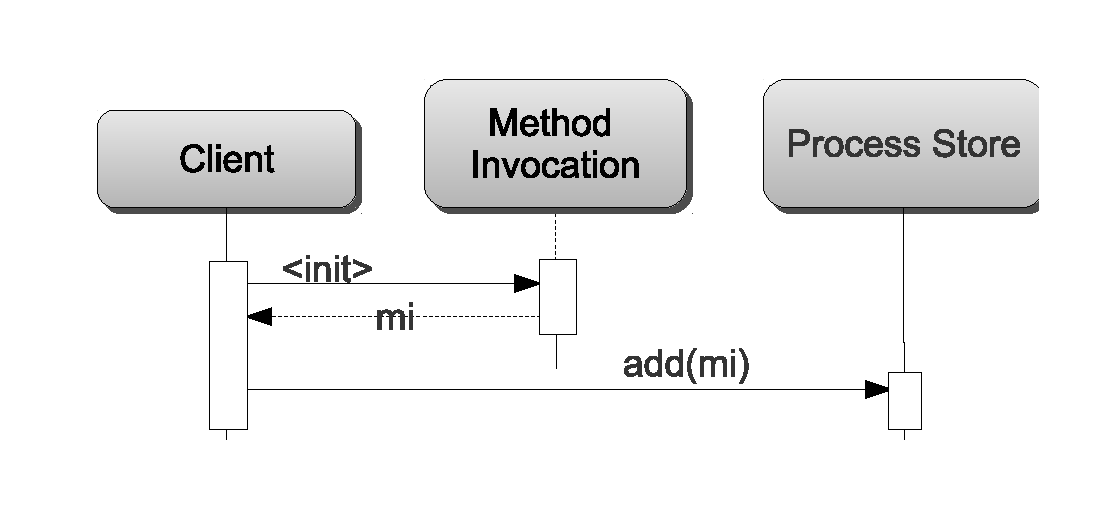
\includegraphics[scale=0.36]{figs/seq-diag-1}
~\\[-3.5cm]ADD:\\[2.5cm]
\caption[New MethodInvocation]{Adding the new MethodInvocations are performed on the Client side.}
\label{fig:add}
%\end{center}
\end{figure}


A method call needs to be sent from the client to the server in an asynchronous way. 
To implement this in Java, the client first constructs an instance of
\MethodInvocation that wraps around the original method call for the server.
Then, 
%the client needs to directly fetch the \ftt{ProcessStore} of the
%server and \ftt{add}s the instance of the method invocation to the server.
%
%Active objects consist of a \texttt{\textbf{ProcessStore}} which stores
% method invocations as described above and a \texttt{\textbf{ExecutionManager}}
% which controls the actual execution of method invocations.
% When an instance of \texttt{\textbf{MethodInvocation}} is created by a client, 
there are two implementation options how to add it to the server's process store:
\begin{enumerate}
  \item The client calls a method on the server to store the instance.
  \item The client directly adds the method invocation into the process
store of the server. 
\end{enumerate}

In option $1$, the server may be busy doing something else. Therefore,
in this case the client must wait until the server is free,  which is
against the asynchronous nature of communication. In Option $2$, the
Java implementation of each active object exposes its process store as
an immutable public property. Thus, the actual code for adding the new
method invocation instance is run in the execution thread of the
client. 
We adopt the second approach as depicted in Figure \ref{fig:add}.
At any time, there can be concurrent clients that are
storing instances of \ftt{MethodInvocation} into the server's process store, but since
the process store implementation encapsulates the mechanisms for concurrency and
data safety, the clients have no concern on data synchronization and concurrency
issues such as mutual exclusion.
The method or policy used to store the method invocation in the process store of
the server is totally up to the server's process store implementation details.
%Storing a method invocation in the process store of the server takes place in
%the client side thread of execution. Listing \ref{lst:jfib_method_fibonacci}
%presents a sample generated Java code for an asynchronous method call in Listing
%\ref{lst:cfib}. 

\subsection{Scheduling the Next Method Invocation}

On the server side of the story,  an active object 
repeatedly fetches an instance of method invocation from its process
store for execution (cf. Fig \ref{fig:take:next}).
The process store uses its instance of
\ftt{SchedulingManager} to choose one of the method invocations. 
\Crisp has some predefined scheduling policies that can be used as scheduling managers;
nevertheless, new scheduling policies can be easily developed
and customized based on the requirements by the user. 
%Listing \ref{lst:aoloop} presents the main loop for the active object. 

\begin{figure}[t]
~\\TAKE:\\
\begin{center}
%\vspace{-1.3cm}
  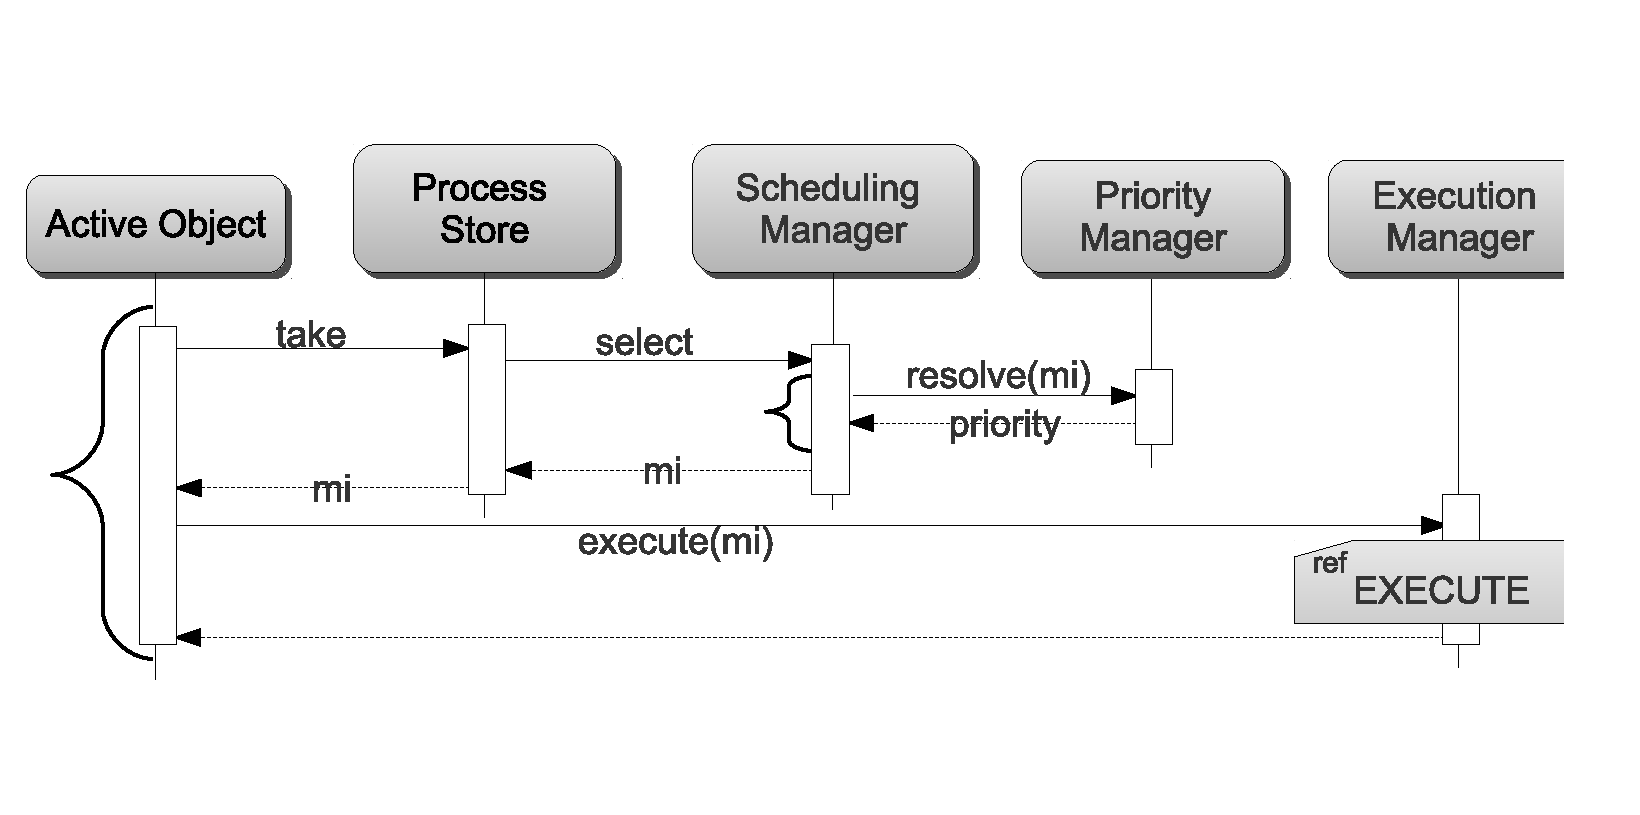
\includegraphics[scale=0.3]{figs/seq-diag-2}
% \vspace{-.7cm}
\end{center}
\caption[Policy-based selection of a MethodInvocation]{An active object selects a method invocation based on its local scheduling policy. After a method finishes execution, the whole scenario is repeated.}
\label{fig:take:next}
\end{figure}

\ftt{SchedulingManager} is an interface the implementations of which
introduce a function to \emph{select} a method invocation based on different
possible criteria (such as time or data) that is either predefined or customized
by the user. The scheduler manager is a component used by process store when
asked to remove and provide an instance of method invocation to be executed.
Thus, the implementation of the scheduling manager is responsible how to choose
one method invocation out of the ones currently stored in the process store of
the active object. Different flavors of the scheduling manager may include
time-based, data-centric, or a mixture.
%\Mahdi{What are concrete examples of scheduling managers?} 
%\Rudi{There is a paper submitted to FMCO post-proceedings about user-defined
%scheduling policies; unfortunately there is no reference to cite yet}

Every method invocation may carry different levels of priority information,
e.g., a server side priority assigned to the method or a
client side priority. 
The \ftt{PriorityManager} 
%is an interface the implementations of which are supposed to 
provides a function to determine and
resolve a final priority value in case there are different levels of priorities
specified for a method invocation. 
% This feature is used, if specified, by the
% process store to compute the ``resolved priority'' of the method invocation
% based on different levels of priorities specified and then add it to the
% storage. 
%An example of a user-defined priority manager is given in Section \ref{sec:caseStudy}.
Postponing the act of resolving priorities to this point rather than when inserting new processes to the store enables us to handle dynamic priorities.


\subsection{Executing a Method Invocation}

To handle processor release points, Creol processes should preserve
their state through the time of awaiting.
This is solved by assigning an instance of a Java thread to each method
invocation. 
An \ftt{ExecutionManager} instance, therefore, employs a ``thread pool''
for execution of its method invocations. 
To create threads, it makes use of the factory pattern:
\ftt{ThreadFactory} is an interface used by the execution manager to
initiate a new thread when new resources are required. 
We cache and reuse the threads so that we can control and tune the performance of resource allocation. 

When a method invocation has to release the processor, its thread must
be suspended and, additionally, its continuation must be added to the
process store. To have the continuation, the thread used for the method
invocation should be preserved to hold the current state; otherwise the
thread may be taken away and the continuation is lost.
The original \ftt{wait} in Java does not provide a way to achieve this
requirement.
Therefore, we introduce \ftt{InterruptibleProcess} as an extension of
\jtt{java.lang.Thread} to preserve the relation.


As shown in Figure \ref{fig:execute}, the thread factory creates threads of type  {\ftt{InterruptibleProcess}}.
The execution manager thread blocks as soon as it starts the interruptible process which executes the associated  method invocation. 
If the method releases the processor before completion, it will be added back to the process store as explained in Section \ref{sec:add}.
When a suspended method invocation is resumed, the execution manager skips the creation of a new thread and  reuses the one that was assigned to the method invocation before.

\begin{figure}[t]
~\\EXECUTE:\\
\begin{center}
% \vspace{-1.3cm}
 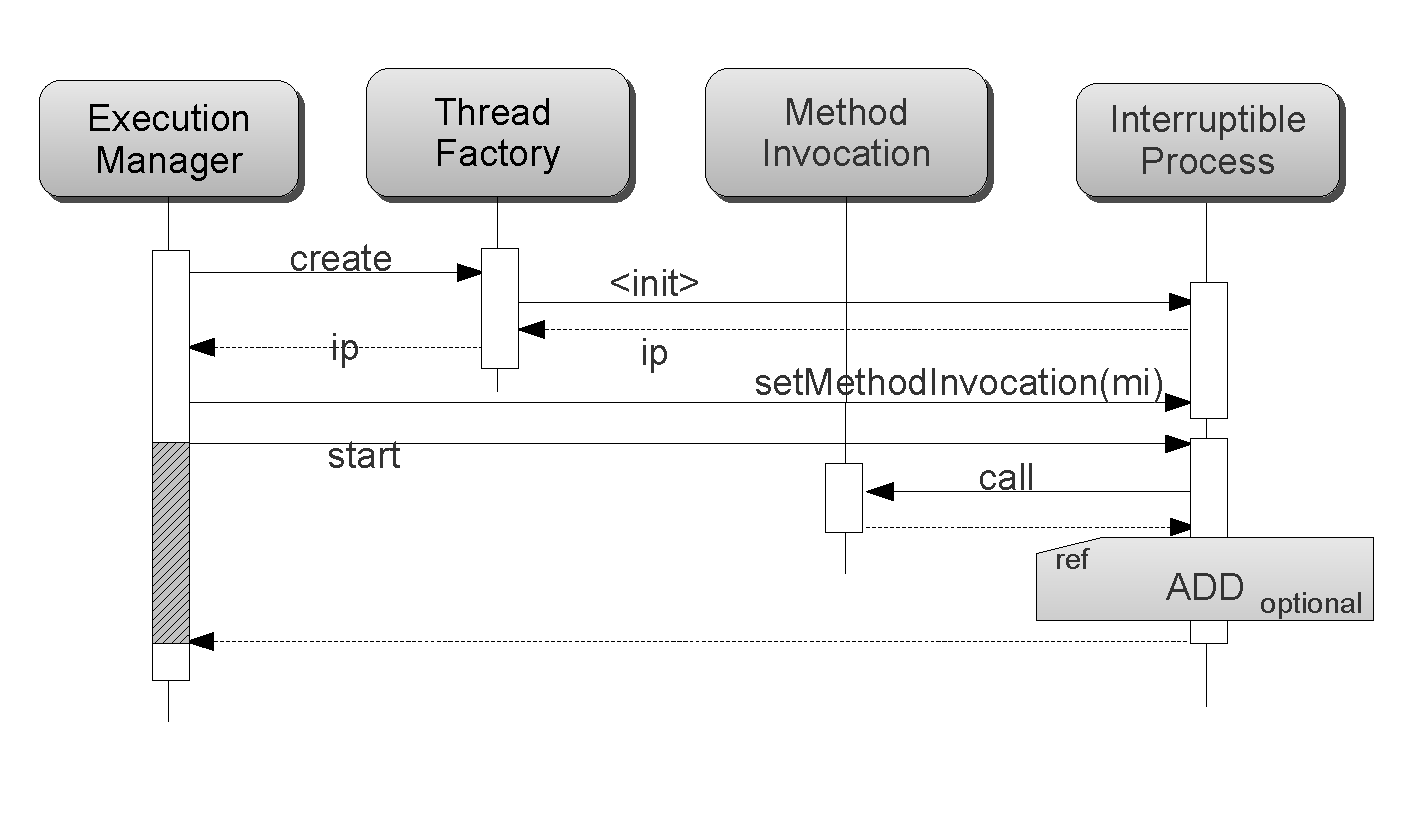
\includegraphics[scale=0.35]{figs/seq-diag-3}
% \vspace{-.7cm}
\end{center}
\caption[Execution of a MethodInvocation]{A method invocation is executed in an interruptible process. The execution manager thread is blocked while the interruptible process is running.}
\label{fig:execute}
\end{figure}


% Our \ftt{ExecutionManager} is an implementation of the standard Java ~interface 
% \jtt{java.util.concurrent.Executor\-Service}. 
% Each active object holds a reference to one execution manager instance.
% Each \ftt{ActiveObject} implements \jtt{java.lang.\-Run\-na\-ble}. So, when
% it gets initialized, it adds \ftt{this} (itself) to
% its execution manager component. This procedure \textit{deploys} the active object
% onto the execution manager corresponding to the underlying multi-core platform.

% FRB: the above last  sentence is not very clear and seems more to hide than to clarify.
% Also the remainder of the section needs to be improved.
% I suggest to add some sequence diagrams.
% Question: when a method invocation executes an await what actually happens to its executing thread?
% Why do we need a thread-pool because only one method at a time is executed?


\subsection{Extension Points}

Besides the methods \ftt{add} and \ftt{take} for adding and removing method invocations, \ftt{ProcessStore} provides methods such as \ftt{preAdd} and \ftt{postAdd} along with \ftt{preTake} and \ftt{postTake} respectively to enable  further customization of the behavior before/after adding or taking a method invocation to/from the store. These extension points enable the customization of priority or scheduling management of the method invocations.

\Crisp provides two generic interfaces for priority specification and scheduling management: \ftt{PriorityManager} and \ftt{SchedulingManager} respectively. These two interface can be freely developed by the programmer to replace the generated code for priorities and scheduling of the messages. It will be the task of the programmer to configure the generated code to use the custom developed classes.

\section{Case Study} \label{sec:caseStudy}

In this section, we demonstrate the use of application-level scheduling and \Crisp with a more complicated example: we program the ``Sieve of Eratosthenes'' %\cite{Sieve_Eratosthenes_wiki}
to generate the prime numbers. 
To implement this algorithm, the 
% \ftt{Sieve} class generates the natural numbers and sends them to the \ftt{Prime} class instances to check whether they can divide these numbers: if a number is not divisible by all primes before that, then it is a new prime number.
% %Initialization of an object happens in its \ftt{init} method, while the \ftt{run} method specifies its active behavior.
% The 
\ftt{Sieve} is initialized by creating an instance of the \ftt{Prime} object representing the first prime number, i.e., \ftt{two}. The active behavior of \ftt{Sieve} consists of generating all natural numbers up to the given limit (100000 in our example) and passing them to the object \ftt{two}. 
A \ftt{Prime} object that cannot divide its input number passes it on to the next \ftt{Prime} object; if there is no next object, then the input number is the next prime and therefore a new object is created.

We parallelize this algorithm by creating active objects that run in parallel.
The numbers are passed asynchronously as a parameter to the \ftt{divide} message. 
Correctness of the parallel algorithm essentially depends on the numbers being processed in increasing order.
For example, if object \ftt{two} processes 9 before 3, it will erroneously treat 9 as a prime, because 3 is not there yet to eliminate 9. 
%Such a scenario is possible if the scheduling of the tasks in the \ftt{Prime} objects is not specified. 
%
To avoid erroneous behavior, we use the actual parameter $n$ in \ftt{divide} method to define its priority level, too (see line \ref{line:priority}). 
As a result, every invocation of this method generates a process with a priority equal to its parameter.
The default scheduling policy for objects always selects a process for execution that has the smallest priority value. 
This guarantees that the numbers sent to a \ftt{Prime} object are processed exactly in increasing order. 

\lstset{language=Creol,escapeinside={(*}{*)}}  
\begin{lstlisting}[float=t, label=lst:prime-sieve-creol, caption=Prime Sieve in Creol]
interface IPrime begin
	op divide(n:Int)
end

class Sieve begin
	var n: Int, two: IPrime
	op init == two := new Prime(2); n := 3
	op run ==
		!two.divide(n);
		if n < 100000 then n := n + 1; !run() end
end

class Prime(p: Int) implements IPrime begin (*\label{lst:priority}*)
	var next: IPrime
	op divide(n: Int) priority (n) == (*\label{line:priority}*)
		if (n % p) /= 0 then 
			if next /= null then
				!next.divide(n)
			else
				next := new Prime(n)
		end end
end
\end{lstlisting}
% 
% class Test
% begin
% 	var g : Sieve
% 	op run == g := new Sieve
% end

We used two different setups to execute the prime sieve program and compare the results. In one setting, we ran the parallel prime sieve compiled by \Crisp; in the other, we executed a sequential program developed based on the same algorithm that uses a single thread of execution in JVM. We performed the experiments on a hardware with $2$ CPU's of each $2$GHz with a main memory of size $2$GB. We ran both programs for $max \in \{10000, 20000, 30000, 50000, 100000\}$.
% We compared two interesting properties of the executions: the thread stack and the number of threads required.

The first interesting observation was that \Crisp prime sieve utilizes all the CPU's on the underlying hardware as much as possible during  execution. 
This can be seen in Figure \ref{fig:multi-cpu-1} which shows the CPU usage. 
Both CPUs are fairly in use while running this program.
Figure \ref{fig:prime_sieve_cacoj} depicts the results of the monitoring of the parallel prime sieve in \Crisp using Visual VM tool. 
It depicts the number of threads generated for the program.
This shows that \Crisp can handle a massive number of concurrent tasks.


One interesting feature of \Crisp is that the execution of any program under \Crisp can constantly utilize the \emph{minimum} memory that can be allocated for each thread in JVM (thread stack). 
In JVM, the size of thread stack can be configured using \ftt{-Xss} option for every run. 
To demonstrate this feature of \Crisp, we collected the minimum stack size needed for every program run in Table \ref{tbl:cmp-thread-stack}. 
All \Crisp runs use the minimum thread stack size of \ftt{64k} that is possible for the JVM.
On the contrary, the stack size required for the sequential version of the sieve program increases by the number of primes detected. 
This is also expected because of the long chain of method calls in the sequential sieve.

% The results depict that the sequential version, through time, increasingly required memory allocation for the thread stack, however, \Crisp performs on a constant size of thread stack. 
% Table \ref{tbl:cmp-thread-stack} summarizes the thread stack allocation on different runs.

\begin{table}[b]\scriptsize
\begin{center}
\begin{tabular}{c c c c c c}
$max$ & $10000$ & $20000$ & $30000$ & $50000$ & $100000$ \\ \thickhline
Sequential & 64k & 72k & 96k & 160k & 190k \\ 
\Crisp & 64k & 64k & 64k & 64k & 64k \\ \thickhline
\end{tabular}
\caption{Thread stack allocated for different executions}
\label{tbl:cmp-thread-stack}
\end{center}
\end{table}

Having the constant thread stack size feature, \Crisp provides another interesting feature. It can handle huge number of thread generation if required. Table \ref{tbl:cmp-thread-num-gen} summarizes the thread generation data for parallel prime sieve in \Crisp. It shows scalability of \Crisp as $p$ rises for parallel prime sieve.
\begin{table}[b]\scriptsize
\begin{center}
\begin{tabular}{c c c}
$max$ & Live Peak & Total \\ \thickhline
$10000$ & 817 & 540591 \\
$20000$ & 1468 & 1854067 \\
$30000$ & 2204 & 4054814 \\
$50000$ & 3707 & 11852985 \\ \thickhline
\end{tabular}
\caption{Number of live threads and total threads created for different runs of parallel prime sieve}
\label{tbl:cmp-thread-num-gen}
\end{center}
\end{table}

As the results show the use of Java threads is costly; first, \Crisp
does not need much of the memory allocated to each thread and, second,
the context switch cost is higher for larger memory allocation. In line
with this, JVM uses a \emph{one-to-one} mapping from an
application-level Java thread to a native OS-level thread. 
In the current setting, the context switch of the threads are in
the OS level. When the context switch is taken to the application
level, we leverage the performance issue from the OS level to the
application level. We further discuss this in Section
\ref{sec:conclusion}.

% In future work, in order to support high numbers of concurrent tasks,
% \Crisp will map a set of Creol messages to one Java thread for each
% active object; thus, indirectly resolving the thread performance
% issue.


\begin{figure}[t]
\begin{center}
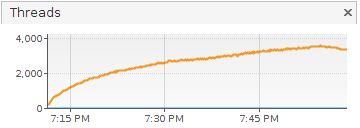
\includegraphics[scale=0.5]{figs/p50000vvm}
\caption{Increasing parallelism in \Crisp for Prime Sieve}
\label{fig:prime_sieve_cacoj}
% \end{center}
% \end{figure}
% 
% \begin{figure}[t]
% \begin{center}
  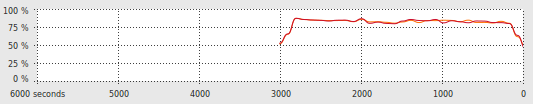
\includegraphics[scale=0.44]{figs/p50000sysmon} 
  \caption{Utilizing both CPUs with Prime Sieve in \Crisp}
  \label{fig:multi-cpu-1}
\end{center}
\end{figure}

\section{Related Work} \label{sec:relwork}
% !TEX root = paper.tex

% Programming multi-core systems is currently a major challenge in software
% engineering. There exist two orthogonal research trends in this area: one
% involves the use of parallel algorithms to solve computational problems faster
% by utilizing multiple cores, e.g., facilitated through functional or declarative
% languages backed by automatic parallelization techniques. Alternatively, as in
% this paper, high-level programming constructs, such as concurrent objects, are
% used at the design stage allowing distributed deployment of  program components
% onto multiple cores. 

% Naturally, employing parallel algorithms inside concurrent
% objects can speed up program execution if more than one core is available for
% each component.

% For multi-core programming, Java has added language support for associating {\em
% tasks} to cores. However, this is in line with the multi-threading paradigm of
% Java which allows different `tasks' on different cores to access shared memory
% (e.g., by calling the methods of the same object). On the contrary, the
% concurrent objects in Creol form a natural basis for deployment on different
% cores; this is similar to actor-based languages, e.g., Scala and Erlang.



The concurrency model of Creol objects, used in this paper, is derived from the
Actor model enriched by synchronization mechanisms and coupled with strong
typing. The Actor model \cite{actors:agha} is a suitable ground for multi-core and distributed 
programming, as objects (actors) are inherently concurrent and autonomous
entities with a single thread of execution which makes them a natural fit for
distributed deployment \cite{actor_frameworks_jvm:agha}. Two successful examples
of actor-based languages are Erlang and Scala. 

Scala is a hybrid object-oriented and functional programming language inspired
by Java. The most important concept introduced in
\cite{scala_actors:ordersky,coord:ordersky} is that Scala Actors unify
\textit{thread-based} and \textit{event-based} programming model to fill the gap
for concurrency programming. Through the event-based model, Scala also
provides the notion of continutations. Scala provides quite the same
features of
scheduling of tasks as in concurrent Java; i.e. it does not provide a direct and
customizable platform to manage and schedule priorities on messages
corresponded among actors.

Erlang \cite{erlang:armstrong} is a dynamically typed functional language that
was developed at Ericsson Computer Science Laboratory with telecommunication
purposes \cite{actors_highly:Correa}. Recent developments in the deployment of
Erlang support the assignment of a scheduler to each processor
\cite{erlang_scheduling} (instead of one global scheduler for the entire
application). This is a crucial improvement in Erlang, because the massive
number of light-weight processes in the asynchronous setting of Erlang turns
scheduling into a serious bottleneck. However, the scheduling policies are not
yet controllable by the application. 

% Such control is quite advantageous for
% further improvement of the overall performance compared to traditional single
% level scheduling at the OS, because scheduling at the OS level is quite more
% expensive. The approach that Erlang adopts provides a coarse-grain base for
% priority scheduling of the messages in the application. Additionally, using the
% notion of light-weight threads, the scheduling is finally delegated to the
% operating system level that rises a bottleneck in message scheduling.

There are well-known efforts in Java to bring in the
functionality of asynchronous message passing onto multicore including Killim
\cite{kilim:Srinivasan_Mycroft}, Jetlang \cite{jetlang}, ActorFoundry
\cite{actor_frameworks_jvm:agha}, and SALSA \cite{salsa:agha} among others. In
\cite{actor_frameworks_jvm:agha}, the authors present a comparative analysis of
actor-based frameworks for JVM platform. However, pertaining to the domain of
priority scheduling of asynchronous messages, all provide a predetermined
approach or a limited control over how message priority scheduling may be at the
hand of the programmer.

% 
% Two competitors of the Actor model in realm of multi-core programming are
% software transactional memory (STM) and data flow programming. Shavit and
% Touitou \cite{stm_shavit_touitou} introduce software transactional memory as a
% method for supporting transactional programming  of synchronized operations.
% They use STM to provide a general concurrent method for translating sequential
% object implementations to non-blocking ones. The most important property of STM
% is its \textit{non-blocking} nature as opposed to lock-based programming models.
% A \textsl{transaction} is finite sequence of local and shared memory machine
% instructions \cite{stm_shavit_touitou}. Transactions are \textit{isolated} and
% \textit{atomic}; the former means that each transactions runs as if others are
% suspended while it runs and the latter means that they are all-or-nothing
% operations \cite{stm_Adl-Tabatabai}. Thus, they give the programmer the illusion
% of a serial execution. \cite{wiki:stm:impl} provides some of the implementations
% of STM in different languages.
% %
% Multiverse \cite{multiverse_homepage} is a Java based STM implementation.
% Clojure \cite{clojure:web,clojure_concurrent:web} provides concurrent programming
% constructs based on STM concepts.
% 
% Data flow programming \cite{dataflow_prog:wiki}, that can be considered a branch
% of flow-based programming \cite{flow_prog:wiki}, focuses on facilitating
% parallel computation through division, conquering and merging of a program based
% on the data on which it processes. Based on data flow programming, in
% \cite{mapreduce:dean_ghemawat}, they propose MapReduce that is basically based
% on one \textit{map} and one \textit{reduce} function. It is originally proposed
% and extensively used at Google. The programmer writes two functions. ``Map''
% takes an input pair and produces a set of intermediate \textsl{key/value} pairs.
% When the computation is done, the library groups together all intermediate
% values associated with the same intermediate key and passes them to reduce
% function. ``Reduce'' function accepts an intermediate key and all the grouped
% associated values and it is supposed to merge the values to possibly form a
% smaller set of values. For instance, in \cite{mapreduce_ml:cheng}, they use
% MapReduce in Machine Learning purposes.

In general, existing high-level languages provide the programmer with little control over
scheduling. The state of the art allows specifying priorities for threads or
processes that are then used by the operating system to order them, e.g.
Real-Time Specification for Java (RTSJ) and Erlang. 
In Crisp, we provide a fine-grain
mechanism which allows for assigning priorities to high-level constructs, e.g., messages and methods.
%between concurrent objects and corresponding application-level intra-object scheduling policies.




Finally, we have considered, in previous work \cite{jaghoori_dating}, local
scheduling policies for Creol objects, with the purpose of schedulability
analysis of real-time models. First of all, this paper is different as it
investigates different levels of priorities that provide a high-level flexible
mechanism to control scheduling. Secondly, we describe at present work how to
compile Creol code to concurrent Java, and by allowing the use of class
libraries
in the underlying framework of Java, we can use Creol as a full-fledged
programming language. % for multi-core programming.



%\begin{table}[t]
%\begin{center}
%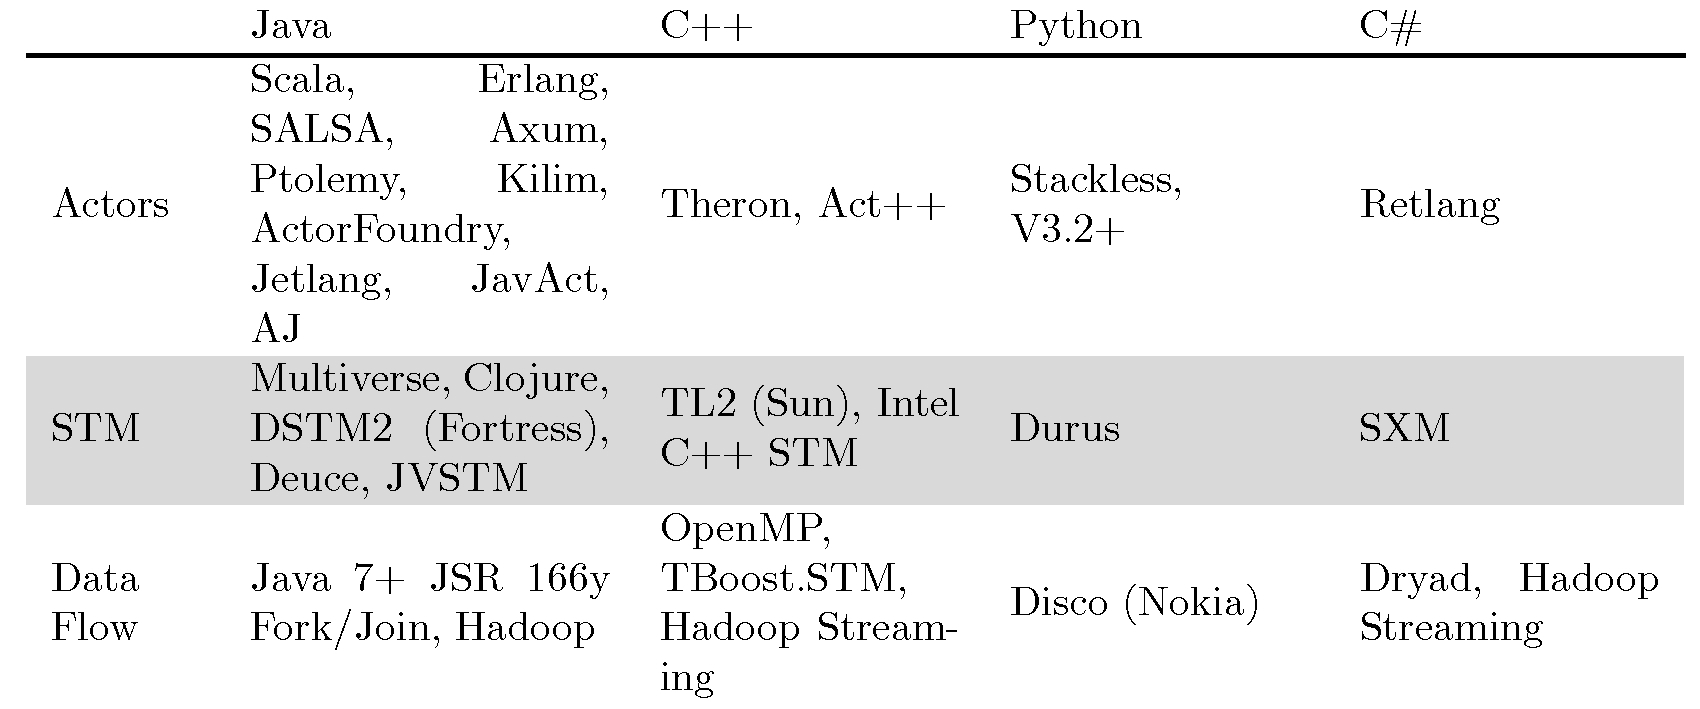
\includegraphics[scale=.85]{langs}
%\caption{Languages and libraries in different paradigms}
%\label{tbl:langs}
%\end{center}
%\end{table}

% SALSA \cite{salsa:agha} is an actor-based
%language for mobile and Internet computing that provides three significant
%mechanisms based on actor model: token-passing continuations, join
%continuations, and first-class continuations. 
%%
%Ptolemy \cite{ptolemy_ii:lee} is
%an actor-oriented open architecture and platform that is used to design, model
%and simulate embedded software. Their approach is hardware software co-design.
%It provides a platform framework along with a set of tools. 
%%
%Axum \cite{axum} is
%a language that builds upon the architecture of the Web and principles of
%isolation, actors, and message-passing to increase application safety,
%responsiveness, scalability, and developer productivity. 
%%
%Kilim \cite{kilim:Srinivasan_Mycroft} is a framework used to create robust and
%massively concurrent actor systems in Java. It uses a bytecode post-processor
%called Weaver \cite{kilim:Srinivasan_Mycroft}. Kilim takes advantage of code
%annotations on bytecode to provide the facility. 
%%
%ActorFoundry
%\cite{actor_frameworks_jvm:agha}] is a Java framework that brings the actor
%model implementation to the developer through the use of code annotations. It
%provides fair scheduling, actor mobility, and safe messaging out of the actor
%semantics. 
%%
%DPJ \cite{dpj} is a project aiming to provide
%deterministic-by-default semantics for an object-oriented, imperative parallel
%language, using primarily compile-time checking.

%
%Multiverse \cite{multiverse_homepage} is a Java based STM implementation that
%aims at seamless integration in the language and language independence in the
%form a framework. Clojure \cite{clojure:web,clojure_concurrent:web} is a dynamic
%programming language as a dialect of LISP that target Java Virtual Machine.
%Clojure provides concurrent programming constructs based on STM concepts. JVSTM
%\cite{jvstm}, another Java based STM library, introduces two core concepts as
%``transactions'' and ``versioned boxes''.
%%The goal is to allow
%% transaction programming at the programming language level, independent of an external
%%transaction manager.

%Java 7 \cite{java7} is supposed to provide language-level features for data flow
%programming as proposed in JSR 166y \cite{jsr166} including fork/join. The
%Apache Hadoop project \cite{hadoop} develops software for reliable, scalable,
%distributed computing proposing several frameworks among which is MapReduce
%\cite{hadoop_mapreduce} that is a framework for distributed processing of large
%data sets on computer clusters.
%
%Act++ \cite{actpp} is a class library for concurrent programming in C++ using
%actors model. Theron \cite{theron} is a lightweight, portable C++ class library
%for developing parallel applications. It implements a simple service-oriented
%model of concurrent processing based on Actor Model.
%
%Intel C++ STM Compiler \cite{intel_cpp_stm_v4} is a C++ platform that provides
%STM concepts of isolation and atomic executions in a C++ compiler. Transactional
%Locking II (TL2) \cite{tl2} is an STM algorithm based on a combination of
%commit-time locking and a novel global version-clock based validation technique.
%TBoost.STM \cite{tboost.stm} is another C++ library that provides STM
%implementation.
%
%The most prominent feature of Stackless Python \cite{stackless_python} is
%\textit{microthreads}, which avoid much of the overhead associated with usual
%Moreover, Python 3.2 \cite{python.3.2} introduces a library for future
%computation based on thread pooling. Durus \cite{durus} is a simple, yet mature,
%complete and fast, STM implementation for Python, allowing both STM inside a
%single process and STM in a server/multiple clients architecture. Disco
%\cite{disco} is a distributed computing framework based on the MapReduce
%paradigm.
%%operating system threads.
%%This avoids many of the overheads of threads, because
%%no mode switching between user mode and kernel mode needs to be done, and can
%%significantly reduce CPU load in some high-concurrency situations.
%
%Retlang \cite{retlang} is intended for use in message based concurrency similar
%to event based actors in Scala. The library does not provide remote messaging
%capabilities. It is designed specifically for high performance in-memory
%messaging.


%%%%%%%%%%%%%%%%%%%%%%%%%%%%%%%%%%%%%%%%%%%%%%%%%%%%%%%%%%%%%%%%%%%%%%%%%%%%%%%%%%%%%%%%%%%%%%%%%%%%

% Agha, in \cite{actors:agha}, introduces ``Actors'' as an inherently concurrent
% programming model. According to \cite{actor_frameworks_jvm:agha}, in the Actor
% model, systems comprise of concurrent and autonomous entities called
% \textit{actors} and \textit{messages}. Actors communicate by sending
% asynchronous messages to other actors for which they should be aware of the
% destination actor \textit{name} (mailbox).
% %Each actor in response to the
% %receiving messages can display different behavior as \cite{actors:agha}
% %proposes:
% %\begin{enumerate}
% %  \item Send a finite set of messages to other known actors;
% %  \item Create a a finite set of new actors; and
% %  \item Define how it will behave in relation to the next incoming messages
% %\end{enumerate}
% %In actor model, there is an extensive usage of ``pattern matching'' for messages
% %that are entrant to the mail box of an actor. This is also important in case of
% %an internal representation of actor. When a programmer is writing an actor, she
% %needs to specify the messages to which the actor will respond. 

% Actor model supporters also tend to take much advantage of ``pattern matching''
% and  ``functional programming'' concepts
% \cite{actors_highly:Correa,erlang:armstrong,salsa:agha,scala_actors:ordersky}.
% \cite{actor_frameworks_jvm:agha} provides a good comparison of the frameworks
% implemented for JVM platform. Moreover, \cite{wiki:actors:impl} provides some of
% the implementing languages and libraries.
% 
% Shavit and Touitou \cite{stm_shavit_touitou} introduce software transactional
% memory as a method for supporting transactional programming  of synchronized
% operations. They use STM to provide a general concurrent method for translating
% sequential object implementations to non-blocking ones. The most important
% property of STM is its \textit{non-blocking} nature as opposed to lock-based
% programming models. A \textsl{transaction} is finite sequence of local and
% shared memory machine instructions \cite{stm_shavit_touitou}. Transactions are
% \textit{isolated} and \textit{atomic}; the former means that each transactions
% runs as if others are suspended while it runs and the latter means that they are
% all-or-nothing operations \cite{stm_Adl-Tabatabai}. Thus, they give the
% programmer the illusion of a serial execution. \cite{wiki:stm:impl} provides
% some of the implementations of STM in different languages.
% 
% %Accordingly, \cite{stm_shavit_touitou} proposes that a software transactional
% %memory is \textit{shared object} that behaves like a memory that supports
% %multiple changes to its addresses by means of transactions. A transaction is a
% %thread of control that applies a finite sequence of primitive operations to
% %memory. This is why software transactional memory is believed to bring in the
% %concept of database transactions on data into object-oriented paradigm. In this
% %model, each object provides a set of \textit{primitive operations} only through
% %which the underlying object (shared memory) can be manipulated. 
% %\cite{stm_shavit_touitou} introduces \textit{wait-free}, \textit{non-blocking},
% %and \textit{swap-tolerant} transactions as types of STM.
% 
% Data flow programming \cite{dataflow_prog:wiki}, that can be considered a branch
% of flow-based programming \cite{flow_prog:wiki}, focuses on facilitating
% parallel computation through division, conquering and merging of a program based
% on the data on which it processes. Based on data flow programming, in
% \cite{mapreduce:dean_ghemawat}, they propose MapReduce that is basically based
% on one \textit{map} and one \textit{reduce} function. It is originally proposed
% and extensively used at Google. The programmer writes two function. ``Map''
% takes an input pair and produces a set of intermediate \textsl{key/value} pairs.
% When the computation is done, the library groups together all intermediate
% values associated with the same intermediate key and passes them to reduce
% function. ``Reduce'' function accepts an intermediate key and all the grouped
% associated values and it is supposed to merge the values to possibly form a
% smaller set of values. For instance, in \cite{mapreduce_ml:cheng}, they use
% MapReduce in Machine Learning purposes.
% 
% Philippsen in \cite{survey_mcp:philippsen} categorizes the problems of
% concurrent object-oriented languages (COOL) as \textit{parallel performance},
% \textit{broken encapsulation}, \textit{inheritance anomalies}, and
% \textit{expressive coordination constraints}. He provides a complete comparison
% of the languages based on the problems; yet the languages used are as of to the
% end of 2000. A more complete of the different concurrent languages can be found
% at \cite{concurrent_lang_list:wiki}.
% %Table \ref{tbl:langs} provides a brief overview of the some of the
% %current languages and libraries. 
% 
% %\begin{table}[t]
% %\begin{center} 
% %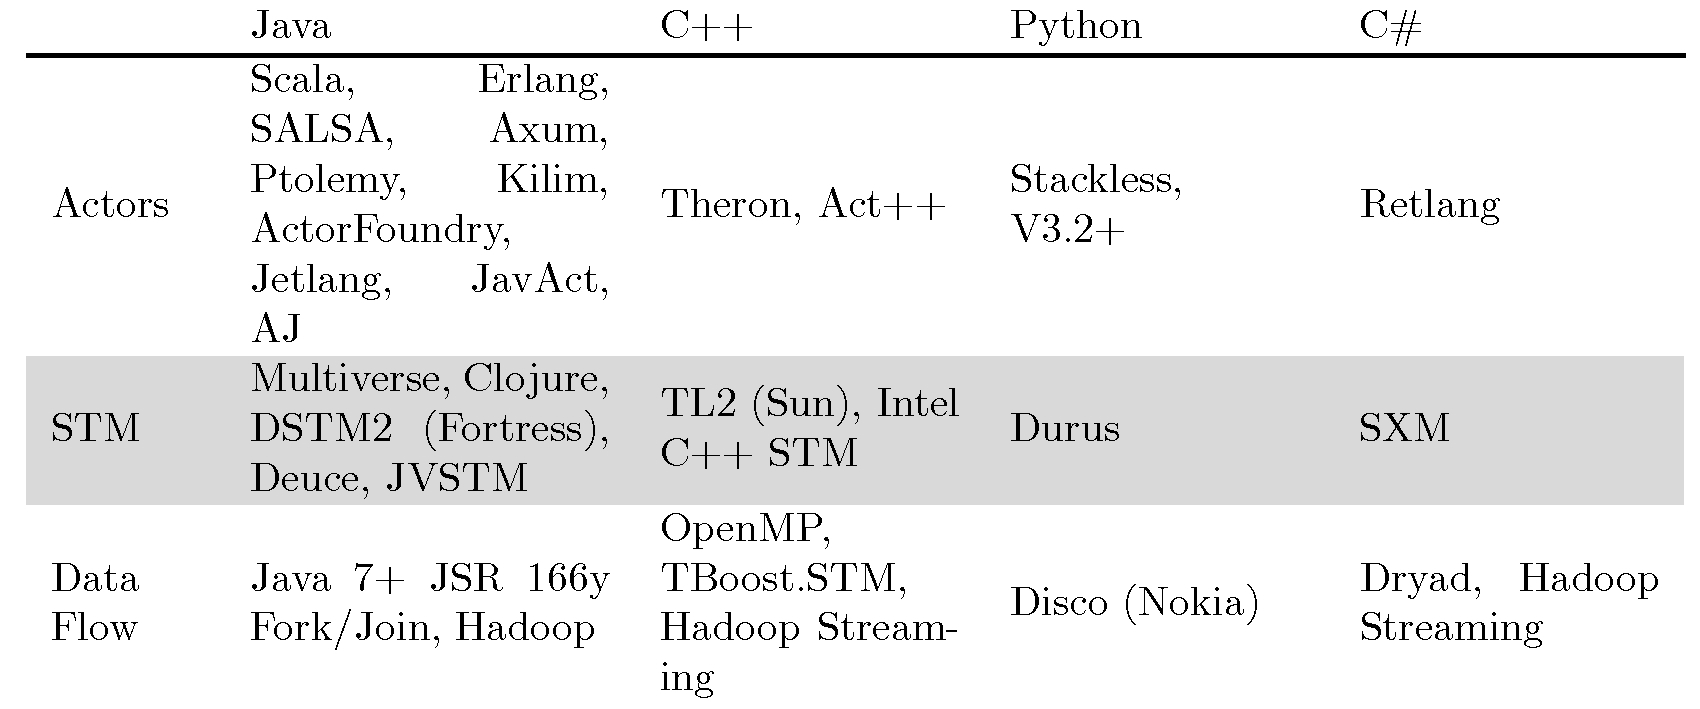
\includegraphics[scale=.85]{langs}
% %\caption{Languages and libraries in different paradigms}
% %\label{tbl:langs}
% %\end{center}
% %\end{table}
% 
% Erlang \cite{erlang:armstrong} is a dynamically typed functional language that
% was developed at Ericsson Computer Science Laboratory with telecommunication
% purposes \cite{actors_highly:Correa}. SALSA \cite{salsa:agha} is an actor-based
% language for mobile and Internet computing that provides three significant
% mechanisms based on actor model: token-passing continuations, join
% continuations, and first-class continuations. Ptolemy \cite{ptolemy_ii:lee} is
% an actor-oriented open architecture and platform that is used to design, model
% and simulate embedded software. Their approach is hardware software co-design.
% It provides a platform framework along with a set of tools. Axum \cite{axum} is
% a language that builds upon the architecture of the Web and principles of
% isolation, actors, and message-passing to increase application safety,
% responsiveness, scalability, and developer productivity. Scala is a hybrid
% object-oriented and functional programming language inspired by Java in which a
% famous Actors library exists that mimics the Erlang implementation. The most
% important concept introduced in \cite{scala_actors:ordersky,coord:ordersky} is
% that Scala Actors unifies \textit{thread-based} and \textit{event-based}
% programming model to fill the gap for concurrency programming.
% %In this model, an
% %actor is a thread that can also \textit{react} to events that come in from other
% %actors; i.e. it provides both \texttt{receive} and \texttt{react} features.
% %\texttt{react} is a complement to \texttt{receive} that is proposed in the
% %original actor model. 
% Kilim \cite{kilim:Srinivasan_Mycroft} is a framework used to create robust and
% massively concurrent actor systems in Java. It uses a bytecode post-processor
% called Weaver \cite{kilim:Srinivasan_Mycroft}. Kilim takes advantage of code
% annotations on bytecode to provide the facility. ActorFoundry
% \cite{actor_frameworks_jvm:agha}] is a Java framework that brings the actor
% model implementation to the developer through the use of code annotations. It
% provides fair scheduling, actor mobility, and safe messaging out of the actor
% semantics. DPJ \cite{dpj} is a project aiming to provide
% deterministic-by-default semantics for an object-oriented, imperative parallel
% language, using primarily compile-time checking.
% %“Deterministic” means that the
% %program produces the same visible output for a given input, in all executions. 
% %“By default” means that deterministic behavior is guaranteed unless the
% %programmer explicitly requests nondeterminism.
% 
% Multiverse \cite{multiverse_homepage} is a Java based STM implementation that
% aims at seamless integration in the language and language independence in the
% form a framework. Clojure \cite{clojure:web,clojure_concurrent:web} is a dynamic
% programming language as a dialect of LISP that target Java Virtual Machine.
% Clojure provides concurrent programming constructs based on STM concepts. JVSTM
% \cite{jvstm}, another Java based STM library, introduces two core concepts as
% ``transactions'' and ``versioned boxes''.
% %The goal is to allow
% % transaction programming at the programming language level, independent of an external
% %transaction manager.
% 
% Java 7 \cite{java7} is supposed to provide language-level features for data flow
% programming as proposed in JSR 166y \cite{jsr166} including fork/join. The
% Apache Hadoop project \cite{hadoop} develops software for reliable, scalable,
% distributed computing proposing several frameworks among which is MapReduce
% \cite{hadoop_mapreduce} that is a framework for distributed processing of large
% data sets on computer clusters.
% 
% Act++ \cite{actpp} is a class library for concurrent programming in C++ using
% actors model. Theron \cite{theron} is a lightweight, portable C++ class library
% for developing parallel applications. It implements a simple service-oriented
% model of concurrent processing based on Actor Model.
% 
% Intel C++ STM Compiler \cite{intel_cpp_stm_v4} is a C++ platform that provides
% STM concepts of isolation and atomic executions in a C++ compiler. Transactional
% Locking II (TL2) \cite{tl2} is an STM algorithm based on a combination of
% commit-time locking and a novel global version-clock based validation technique.
% TBoost.STM \cite{tboost.stm} is another C++ library that provides STM
% implementation.
% 
% The most prominent feature of Stackless Python \cite{stackless_python} is
% \textit{microthreads}, which avoid much of the overhead associated with usual
% Moreover, Python 3.2 \cite{python.3.2} introduces a library for future
% computation based on thread pooling. Durus \cite{durus} is a simple, yet mature,
% complete and fast, STM implementation for Python, allowing both STM inside a
% single process and STM in a server/multiple clients architecture. Disco
% \cite{disco} is a distributed computing framework based on the MapReduce
% paradigm.
% %operating system threads. 
% %This avoids many of the overheads of threads, because
% %no mode switching between user mode and kernel mode needs to be done, and can
% %significantly reduce CPU load in some high-concurrency situations. 
% 
% Retlang \cite{retlang} is intended for use in message based concurrency similar
% to event based actors in Scala. The library does not provide remote messaging
% capabilities. It is designed specifically for high performance in-memory
% messaging.
% 
% %\subsection{Discussion}
% %
% %Many of the well-known languages provide language constructs enabling the
% %programmer to take advantage of multicore technology. The language features
% %include concepts such as conditions, atomic data structures, and locks among
% %others. They all provide the required fundamentals to build more complex data
% %structures and programs that need to take advantage of concurrent objects on
% %multicore. Though, they also introduce new challenges in accordance: 
% %
% %\begin{description}
% %  \item[Level of abstraction.] Although the language constructs for multicore
% %  are based on a high-level paradigm such as object orientation, they seem to be
% %  still in lower levels of abstraction expected for multicore. In other words,
% %  the current feature set provide sound primitives for programming multicore
% %  yet to grow mature to higher level of abstraction for simpler use.
% %  \item[Composability.] Another interesting challenge of using language
% %  primitives to construct concurrent objects is how to use them in use cases of
% %  composition to build larger programs. Composing pieces of code to build
% %  larger code often bring in the problem of complexity. The complexity in this
% %  area rises up in the form of synchronization issues required to be resolved by
% %  the programming technique adopted by the programmer. In this line, Aka
% %  (REF???) is an interesting attempt to create a hybrid solution to alleviate the
% %  challenges.
% %  \item[Level of expertise.] Generally speaking, it is the responsibility of the
% %  programmer to come up with a correct and efficient design how to use the
% %  language fundamental features to build a more complicated program. In essence,
% %  this capability depends on the level of experience, skill, and knowledge
% %  of programming concepts. It is more desirable to propose and provide
% %  higher-level yet simpler programming language constructs so that the
% %  programmer can easily take advantage with little concern on the level of expertise
% %  required to use them.
% %\end{description}
% %
% %In another line of research efforts, libraries have been developed to provide a
% %solution on top of a language for concurrent objects on multicore. Development
% %of libraries give rise to concerns:
% %\begin{description}
% %  \item[Side Effects.] Usually the compiler of the language does not know
% %  about the semantics of the added library meaning that it may bring side
% %  effects to the correctness of the executing code \cite{survey_mcp:philippsen}.
% %  \item[Compiler Optimizations.] In another insight into library development,
% %  the compiler optimization process is missed out for the extra code since the
% %  compiler is not accordingly instrumented to act upon the new code for the
% %  added library \cite{survey_mcp:philippsen}. Optimizations may become important
% %  in case of heavy processing needs or limitations of resources.
% %  \item[Coverage.] Another interesting point in library development is that
% %  libraries are \textit{usually} developed with specific directions or concerns.
% %  This means that they do not consider all the concerns in concurrent objects
% %  concepts for the purpose of simplicity or prototyping 
% %  \cite{survey_mcp:philippsen}.
% %\end{description}
% 
% 
% 


\section{Conclusion} \label{sec:conclusion}
In this paper, we proposed \Crisp as an implementation scheme for
application-level scheduling of active objects. 
\Crisp first introduces asynchronous message passing with fine-grain
priority management and scheduling of messages. 
Additionally, it introduces a Creol to Java compiler that translates
the active objects in Creol into an equivalent Java application. 
\Crisp compiler seamlessly integrates Java class libraries into Creol
including data types that turns Creol from a modeling language to a
fully-fledged one in the hands of the programmer. 
% \Crisp compiler takes advantage of template engines; i.e. the code
% generation templates can easily be customized in the direction of the
% requirements of the problems at hand.

The \jtt{java.util.\-con\-current} package provides useful API for
concurrent programming. Java futures facilitate modeling
asynchronous message passing. However, for processor release
points, we had to preserve threads (using \jtt{Interruptible\-Process})
to allow continuations which leads to their OS-level context switching
that is costly. Moreover, we were tightly directed to use the
out-of-the-box \jtt{Executor\-Service} which is limitedly extensible. We
had no control over the scheduling mechanisms of the internal queue used
in the service implementations. Thus, we needed to re-implement some of
the concepts. Through prototyping \Crisp, we learned that
there are two major
challenges ahead. Firstly, we need to integrate continuations into Java
using a many-messages-to-one-thread mapping model. Secondly, we need
complete control over scheduling of messages and threads in
\jtt{Executor\-Service}'s internal queue. Table \ref{tbl:eval}
summarizes this discussion.

\begin{table}[h]\small
\begin{center}
\begin{tabular}{p{1.5cm} p{2cm} p{2cm} p{1.5cm}}
 & Asynchronous Communication & Processor Release Point & Scheduling \\
\thickhline
Modeling & \ding{51} & \ding{51} & \ding{53} \\
Performance & \ding{51} & \ding{53} & \ding{51} \\ \thickhline
 & Java Futures & Interruptible Process & Executor Service \\
\end{tabular}
\caption{Overview of evaluation of challenges}
\label{tbl:eval}
\end{center}
\end{table}


In future, we will focus on thread performance
for \Crisp such that thread scalability can be achieved to a certain
limit. Additionally, the development of concurrency features on
multi-core in \Crisp is one of the major future concentrations.
% We will extend Creol to provide the necessary syntax to express all
% different levels of priorities.
% including method level, message level, and object level priorities. 
Moreover, another line of future work involves profiling and monitoring
objects  at runtime  to be used for optimization and performance
improvement.
In addition, we intend to extend and integrate into our tool set 
model checking engines such as Modere \cite{JaghooriMS06}.

% \bibliographystyle{plain}
% \bibliography{references}

% Local Variables:
% fill-column: 80
% End:

\lstset{escapeinside={}{}}
